%%%%%%%%%%%%%%%%%%%%%%%%%%%%%%%%%%%%%%%%%%%%%%%%%%%%%%%%%%%%%%%%%%%%%%%%%
% This file is part of the LaTeX sources of the OMDoc 1.6 project descriptions
% Copyright (c) 2006 A.M. Cohen, H. Cuypers, E. Reinaldo Barreiro
% This work is licensed by the Creative Commons Share-Alike license
% see http://creativecommons.org/licenses/by-sa/2.5/ for details
% The source original is at https://github.com/KWARC/OMDoc/doc/projects/mathdox2
%%%%%%%%%%%%%%%%%%%%%%%%%%%%%%%%%%%%%%%%%%%%%%%%%%%%%%%%%%%%%%%%%%%%%%%%%

\begin{omgroup}[id=mathdox2,short=MathDox,creators={amc,cuypers,barreiro}]
                        {MathDox: Mathematical Documents on the Web}
\ednote{project page: \url{http://www.mathdox.org}}

\renewcommand{\CAS}{\indextoo{CAS}}


The {\MathDox} system provides an infrastructure for
{\atwintoo{interactive}{mathematical}{document}s} that make use of the World Wide Web.
These documents take input from various sources, users, and mathematical services.
Communication between these different entities can be realized using {\openmath}.  But,
such {\indextoo{communication}} and the {\indextoo{interactivity}} inside the mathematical
document take place in a specific, dynamic context. In this paper we discuss our approach
to such a {\atwintoo{dynamic}{mathematical}{context}}: {\MathDox}.  It consists of both an
{\xml}-based markup language for interactive mathematical contents and a set of software
tools realizing the interactivity.

\begin{omgroup}{Introduction}
Although the notion of an interactive mathematical document has been around for several
years, cf.~\cite{CohMee:tapap98}, its realization is nowhere near the final stage. For
instance, recent progress in web technologies has enabled a much smoother communication of
mathematics than ever before. The use of an interactive mathematical document (IMD) can
provide a window to the world of mathematical services on the Internet, and a mathematical
service on the Internet can be created by the building of an interactive mathematical
document.  {\MathDox} is an ensemble of software tools for creating IMDs, it includes
\begin{enumerate}
\item an {\xml} based language that offers markup support for the source texts of IMDs;
\item a document server, rendering interactive mathematical documents from source text and
  interactively obtained information;
\item mathematical services, providing connections with {\CAS{s}} like {\mathematica} and
  {\gap} via {\openmath} phrasebooks (cf.~\cite{URL:omsoc}).
\end{enumerate}

The creation of {\MathDox} is a project at the Technische Universiteit Eindhoven (the
RIACA institute).  Several people at RIACA have helped creating it; here we mention
Manfred Riem, Olga Caprotti, Hans Sterk, Henny Wilbrink, Mark Spanbroek, Dorina Jibetean.
The system is mainly built with Java and related technology.  The products are available
via the project web site and will be licensed under the Lesser Gnu Public
License~\cite{LGPL}.
\end{omgroup}

\begin{omgroup}[id=mathdox.ui]{The Language}
The \MathDox\ source is an \xml\ document.  We have derived our own document type
definitions (DTD) for these source texts.  We have been influenced by both
{\docbook}~\cite{WalMue:dtdg99} and {\omdoc}. The former is a fairly general standard for
electronic books, the latter is a very rich, and strongly logic-oriented standard for
mathematical documents---the main subject of this book.  Both {\omdoc} and {\MathDox} use
{\openmath}~\cite{BusCapCar:2oms04}, the difference being that {\omdoc} focuses on
representing mathematical knowledge whereas {\MathDox} focuses on interactivity.  The
connections with both DocBook and {\omdoc} are of importance to us because we expect
several authoring tools for it to emerge in the coming few years, and we want to profit
from their presence.

The mathematics in the {\MathDox} source is given by means of {\openmath} objects.  This
feature has clear advantages in terms of portability. The DocBook type grammar sees to it
that there are natural scopes, where mathematical objects `live'. For instance, when a
chapter begins with ``Let $\mathbb{F}$ be a field'', the scope of the variable
$\mathbb{F}$ is assumed to be the whole chapter (although, somewhere further down the
hierarchy, say in a section of the chapter, this assignment can be overridden).

Interactivity in {\MathDox} is taken care of by {\xml} tags representing various
{\twintoo{programming}{construct}s} as well as queries to
{\atwintoo{external}{mathematical}{service}s}.  These actions take place within part of
the context, which fixes the precise semantics of the objects involved.  Further
constructs are available for handling context and user input.  Our notion of context is
based on \cite{FraHes:aoidms99}. Context is divided into static\twin{static}{context} and
{\twintoo{dynamic}{context}}. The static context may be defined as the set of all {\xml}
sources from which a interactive document can be prepared for use. Two extreme forms are
{\openmath} Content Dictionaries\twin{content}{dictionary} and a chapter of an ordinary
book.  The dynamic context behaves more like the {\indextoo{state}} of a {\CAS}.  It
keeps track of the variables introduced, their properties, their values, and their scopes.
The {\MathDox} language has constructs for storing and changing this information.  For
example, the field $\mathbb{F}$ introduced at the beginning of a chapter may be specified
to be a finite field of five elements in the context of a particular section of the
chapter.

Although semantics is the primary target, some features for presentation have been built
into the language.  In order to have a flexible presentation, we use
presentation-annotated {\openmath}.  In \MathDox\ we allow style attributes inside
{\openmath} objects.  By discarding these style attributes, regular {\openmath} is
obtained. For instance, by providing the appropriate value for the style attribute, the
author has a choice between a slash and a fraction display. In $\frac{3/4+2/3}{5}$ we have
used them both.

Another way of solving presentation issues is illustrated by the statement:
$3,4\in\mathbb{Z}$.  The corresponding {\openmath} expression would be the equivalent of
$3\in\mathbb{Z} \wedge 4\in\mathbb{Z}$, but our {\openmath} statement reads that the
sequence $3,4$ belongs to $\mathbb{Z}$.  So here, the semantics of the element-of symbol
has been stretched so as to help out presentation.
\end{omgroup}

\begin{omgroup}[id=mathdox.cont_theory]{The {\MathDox} System}

An essential component of the {\MathDox} software is its {\twintoo{document}{server}}. It
provides a view to the client of the content and manages both the
static\twin{static}{context} and the {\twintoo{dynamic}{context}}.  The usage of the
{\MathDox} document server is shown in {\myfigref{DocModel}}. We explain in some detail
the main components shown in this picture.


\begin{myfig}{DocModel}{The {\MathDox} software}
  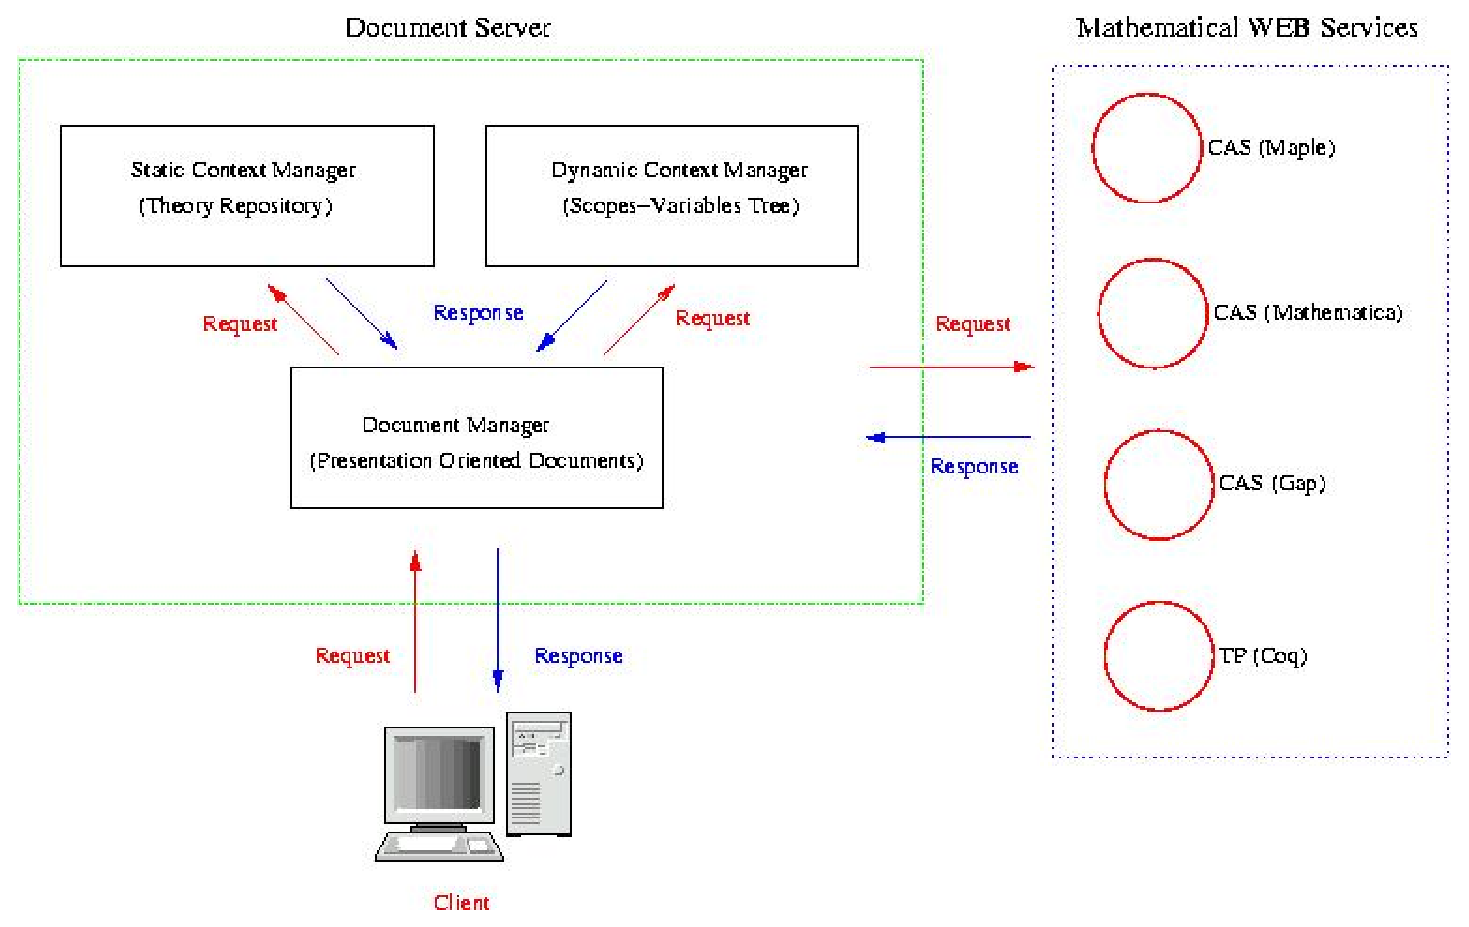
\includegraphics[width=11cm]{\projectsPath{mathdox/DocModel}}
\end{myfig}

\begin{enumerate}
\item The {\emph{client}}. The client is realized by a
  {\atwintoo{math-enabled}{web}{browser}}.  It will present views of the documents served
  to the user, interact with the user, and communicate user input to the document server.

  The communication between client and server takes place via the HTTP request/response
  mechanism.  The responsibility for interaction is mostly on the server side.
\item The {\emph{\twintoo{document}{server}}}.  This server caters for presentation,
  communication, and context.  It supports a wide range of actions ranging from handling
  queries to searching within documents for mathematical content and from placing (and
  retrieving) objects into the context, to rendering documents in different views.

  The document server is realized as a Java enhanced
  {\twintoo{web}{application}}~\cite{URL:jsp} inside a web server.  It is not a monolithic
  entity. As shown in {\myfigref{DocModel}}, it is formed by the system parts.  The
  {\emph{\twintoo{document}{manager}}} serves views to the client.  IMDs can be thought of
  as programs (scripts) encoding the production of a response.  In generating the
  response, they can make use of the information contained in the static context, and in
  the dynamic context (scopes and variables), the user input communicated along with
  request, and the results of computations carried on by one or more mathematical
  services.
  
  Another part is the {\emph{\atwintoo{static}{context}{manager}}} which is responsible
  for managing a repository of {\MathDox} mathematical theories.
  
  The final (third) part is the {\emph{\atwintoo{dynamic}{context}{manager}}} which is
  responsible for the dynamic information.

\item {\em\twintoo{mathematical}{service}s}.  Mathematical services can be very diverse:
  some may serve as general interfaces to {\CAS} or to Theorem Provers.  The {\MathDox}
  software provides ways to access these services via standard protocols, among which
  those developed under the MONET project~\cite{URL:monet}.  The mechanism extends the
  phrasebook set-up for {\openmath}~\cite{CapCoh:uosdmc00,CapCoh:jpcaad00}.  For
  constructing specific {\openmath} services, we employ our Java {\openmath} library
  ROML~\cite{URL:roml}.
\end{enumerate}
\end{omgroup}

\begin{omgroup}{Conclusion}
Now that {\MathDox} is close to a complete working version, trial applications are in the
make. We mention
\begin{itemize}
\item a server for providing designs of experiments on command to statisticians,
\item an exercise repository for the EU funded LeActiveMath project,
\item a mathematics course on calculus, with automated natural language production from a
  formal-mathematical source for the EU funded project WebALT,
\item interactive lecture notes (the successor of~\cite{CohCuySterk:ida99}) for an
  Abstract Algebra course within a mathematically oriented Bachelor curriculum,
\item educational material for highschool mathematics in the Netherlands.
\end{itemize}
\end{omgroup}
\end{omgroup}
%%% Local Variables: 
%%% mode: latex
%%% TeX-master: "../main"
%%% End: 

% LocalWords:  MathDox mathdox Cuypers Barreiro Eindhoven IMD IMDs CAS DocBook
% LocalWords:  cf phrasebooks Technische Universiteit RIACA Riem Caprotti Sterk
% LocalWords:  Henny Wilbrink Spanbroek Dorina Jibetean DTD HTTP phrasebook ath
% LocalWords:  ROML LeActiveMath WebALT highschool hrasebooks omputer lgebra pp
% LocalWords:  utomated eduction SIGSAM Rom Arjeh ATCM Chiang Chu Jen Chuan eds
% LocalWords:  ISBN Meertens ACELA Kajler Wien JavaServer Franke Ch Sorge vol
% LocalWords:  sk mathdox DocModel mathdox mathdox mathdox mathdox
